\documentclass{standalone}

\usepackage{tikz}
\usetikzlibrary{arrows}
\usetikzlibrary{decorations.markings}
\usepackage{standalone}

\begin{document}

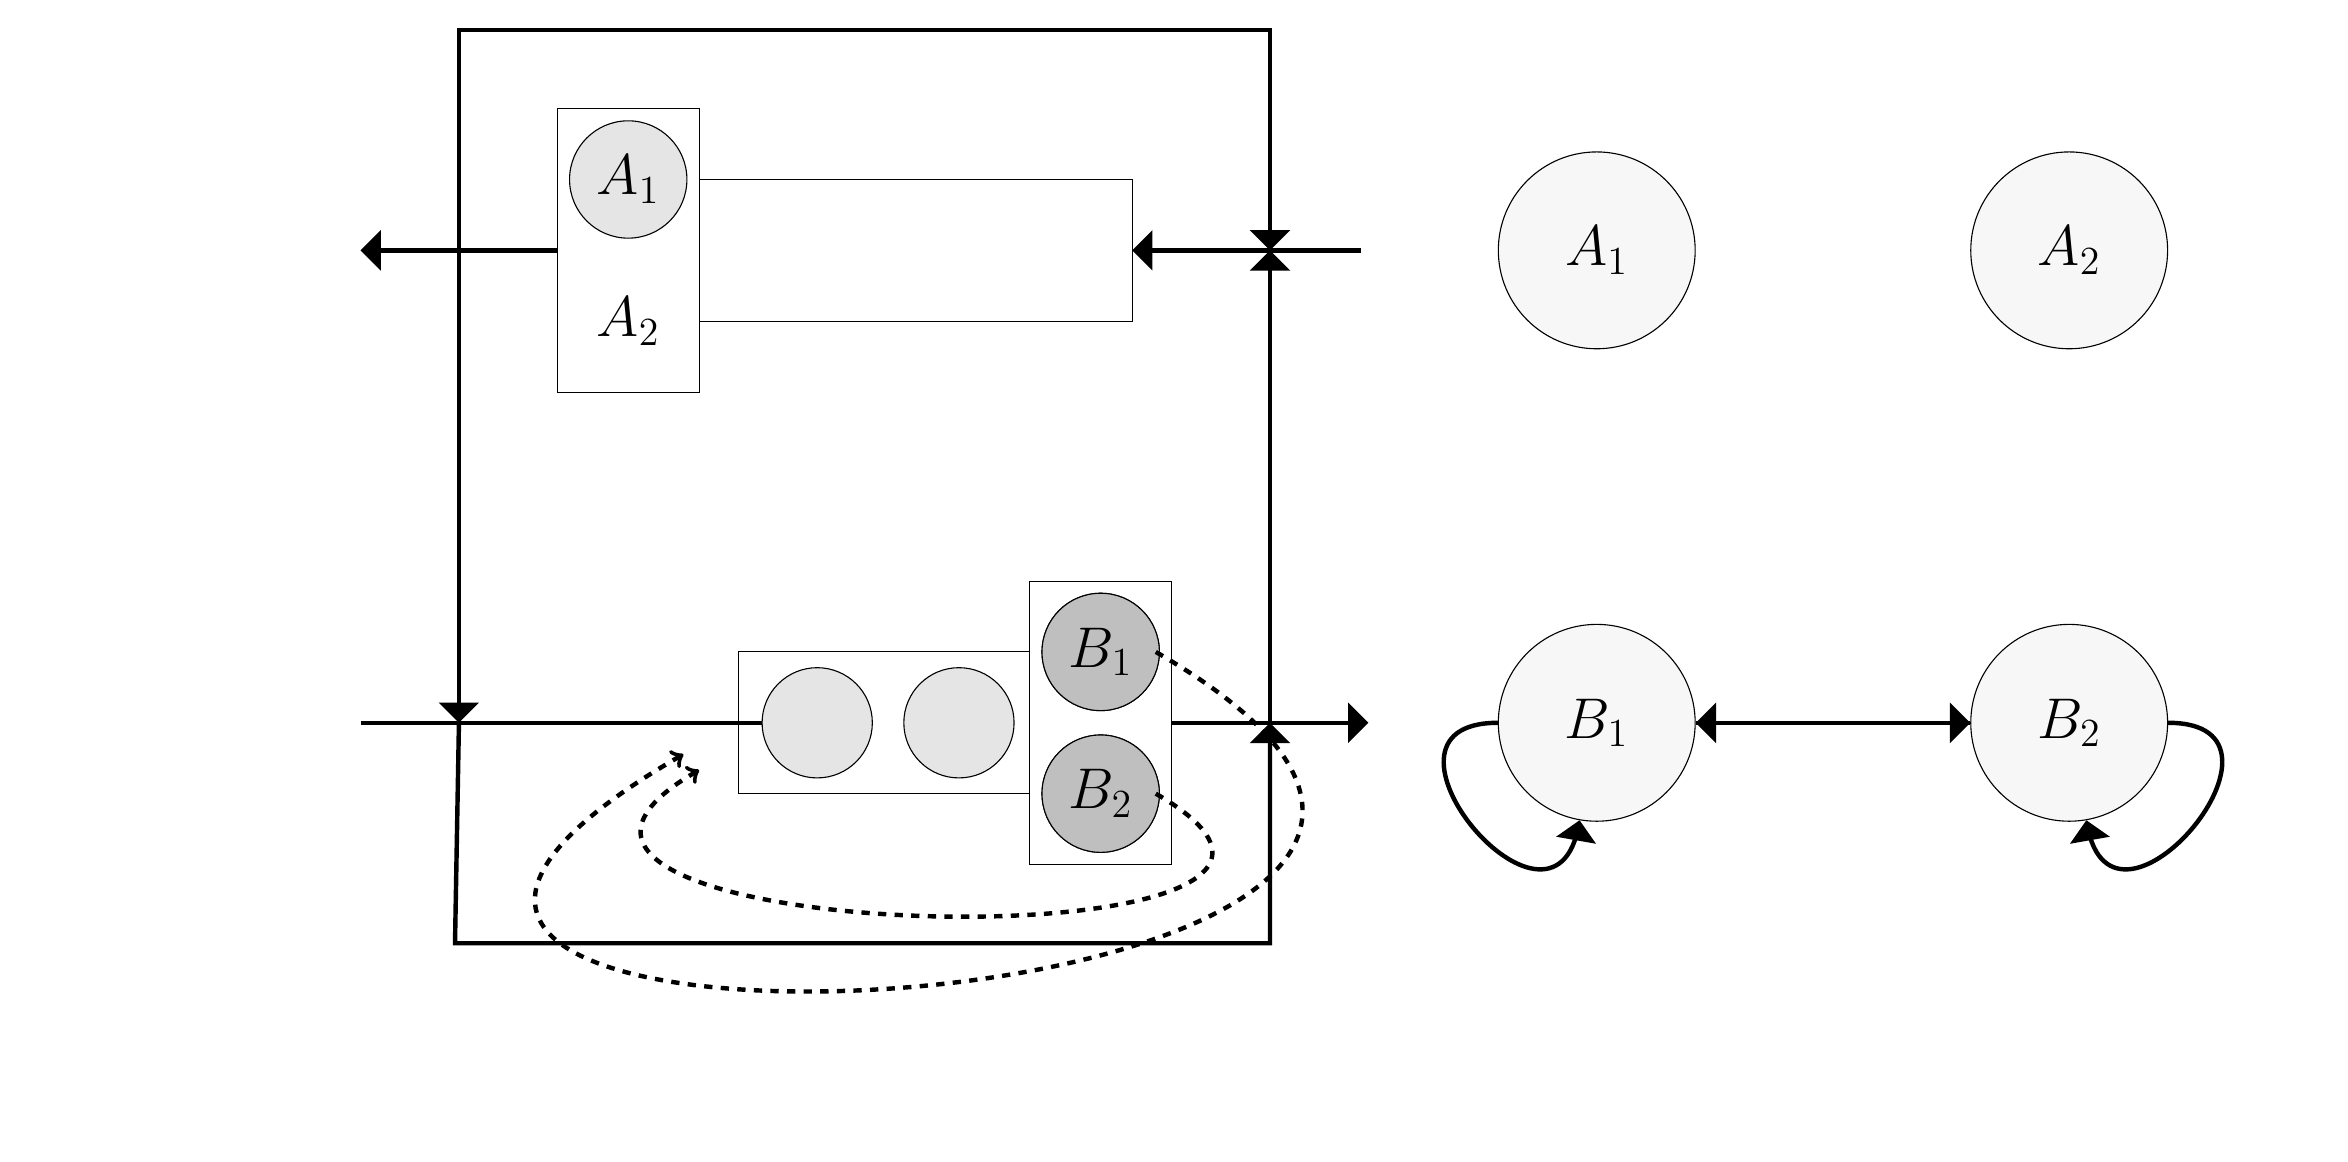
\begin{tikzpicture}

% Node bottom
\draw (-4.9, 2.1) rectangle (-1.2, 3.9);
\draw (-1.2, 1.2) rectangle (0.6, 4.8);

% Nodes middle
\draw (-5.4, 8.1) rectangle (0.1, 9.9);
\draw (-7.2, 7.2) rectangle (-5.4, 10.8);

% Routings
\draw[ultra thick, -triangle 90] (3, 9) -- (0.1, 9); % middle to middle
\draw[ultra thick, -triangle 90] (-7.2, 9) -- (-9.7, 9); % out of middle

\draw[ultra thick, -triangle 90] (-9.7, 3) -- (-3.9, 3); % In to bottom
\draw[ultra thick, -triangle 90] (0.6, 3) -- (3.1, 3); % Out of bottom

\draw[ultra thick, -triangle 90] (-8.45, 9) -- (-8.45, 3); % middle to bottom
\draw[ultra thick, -triangle 90] (1.85, 3) -- (1.85, 9); % bottom to middle

\draw[ultra thick, -triangle 90] (-8.45, 9) -- (-8.45, 11.8) -- (1.85, 11.8) -- (1.85, 9); % top left to top right
\draw[ultra thick, -triangle 90] (-8.45, 3) -- (-8.5, 0.2) -- (1.85, 0.2) -- (1.85, 3); % bottom loop


% middle left
\node[align=center] [style={minimum size=1.4cm, text width=1.0cm, draw=black,fill=black!10,text=black,shape=circle}] at (-6.3, 9.9) {\huge $A_1$};
% \node[align=center] [style={minimum size=1.4cm, text width=1.0cm, draw=black,fill=black!10,text=black,shape=circle}] at (-6.3, 8.1) {\huge $A_2$};
\node[align=center] [style={minimum size=1.4cm, text width=1.0cm, draw=none,fill=none,text=black,shape=circle}] at (-6.3, 8.1) {\huge $A_2$};
% \node[align=center] [style={minimum size=1.4cm, text width=1.0cm, draw=black,fill=black!10,text=black,shape=circle}] at (-4.5, 9) {};
% \node[align=center] [style={minimum size=1.4cm, text width=1.0cm, draw=black,fill=black!10,text=black,shape=circle}] at (-2.7, 9) {};
% \node[align=center] [style={minimum size=1.4cm, text width=1.0cm, draw=black,fill=black!10,text=black,shape=circle}] at (-0.9, 9) {};

% Bottom customers
\node[align=center] [style={minimum size=1.4cm, text width=1.0cm, draw=black,fill=black!10,text=black,shape=circle}] at (7.2-7.5, 3.9) {\huge $B_1$};
\node[align=center] [style={minimum size=1.4cm, text width=1.0cm, draw=black,fill=black!10,text=black,shape=circle}] at (7.2-7.5, 2.1) {\huge $B_2$};
\node[align=center] [style={minimum size=1.4cm, text width=1.0cm, draw=black,fill=black!10,text=black,shape=circle}] at (3.6-7.5, 3) {};
\node[align=center] [style={minimum size=1.4cm, text width=1.0cm, draw=black,fill=black!10,text=black,shape=circle}] at (5.4-7.5, 3) {};

% State digraph Nodes


\node (A1) [style={minimum size=2.5cm,draw=black,fill=black!3,text=black,shape=circle}] at (6, 9) {\huge{$A_1$}};
\node (A2) [style={minimum size=2.5cm,draw=black,fill=black!3,text=black,shape=circle}] at (12, 9) {\huge{$A_2$}};
\node (B1) [style={minimum size=2.5cm,draw=black,fill=black!3,text=black,shape=circle}] at (6, 3) {\huge{$B_1$}};
\node (B2) [style={minimum size=2.5cm,draw=black,fill=black!3,text=black,shape=circle}] at (12, 3) {\huge{$B_2$}};


% B2 to B
\node[align=center] [style={minimum size=1.4cm, text width=1.0cm, draw=black,fill=black!25,text=black,shape=circle}] at (7.2-7.5, 2.1) {\huge $B_2$};
\draw[ultra thick, -triangle 90] (B2) -- (B1);
\draw[ultra thick, -triangle 90] (B2) [out=0, in=-80, looseness=3] to (B2);
\draw[ultra thick, black, dashed, ->] (7.9-7.5, 2.1) [out=-30, in=-150, looseness=2] to (-5.4, 2.4);

% B1 to B
\node[align=center] [style={minimum size=1.4cm, text width=1.0cm, draw=black,fill=black!25,text=black,shape=circle}] at (7.2-7.5, 3.9) {\huge $B_1$};
\draw[ultra thick, -triangle 90] (B1) [out=180, in=-100, looseness=3] to  (B1);
\draw[ultra thick, -triangle 90] (B1) -- (B2);
\draw[ultra thick, black, dashed, ->] (7.9-7.5, 3.9) [out=-30, in=-150, looseness=4] to (-5.6, 2.6);




\end{tikzpicture}

\end{document}